\section{Procrustes Analysis}~\label{sec:procrustes}
Beyond just studying how individual sentiments have changed over time,
we also sought to study how the \emph{overall} conversation shifts.
To do this, we used \emph{procrustes analysis} to compare the
word embeddings of conversatiosn across different years.

\begin{figure}[H]
  \centering
  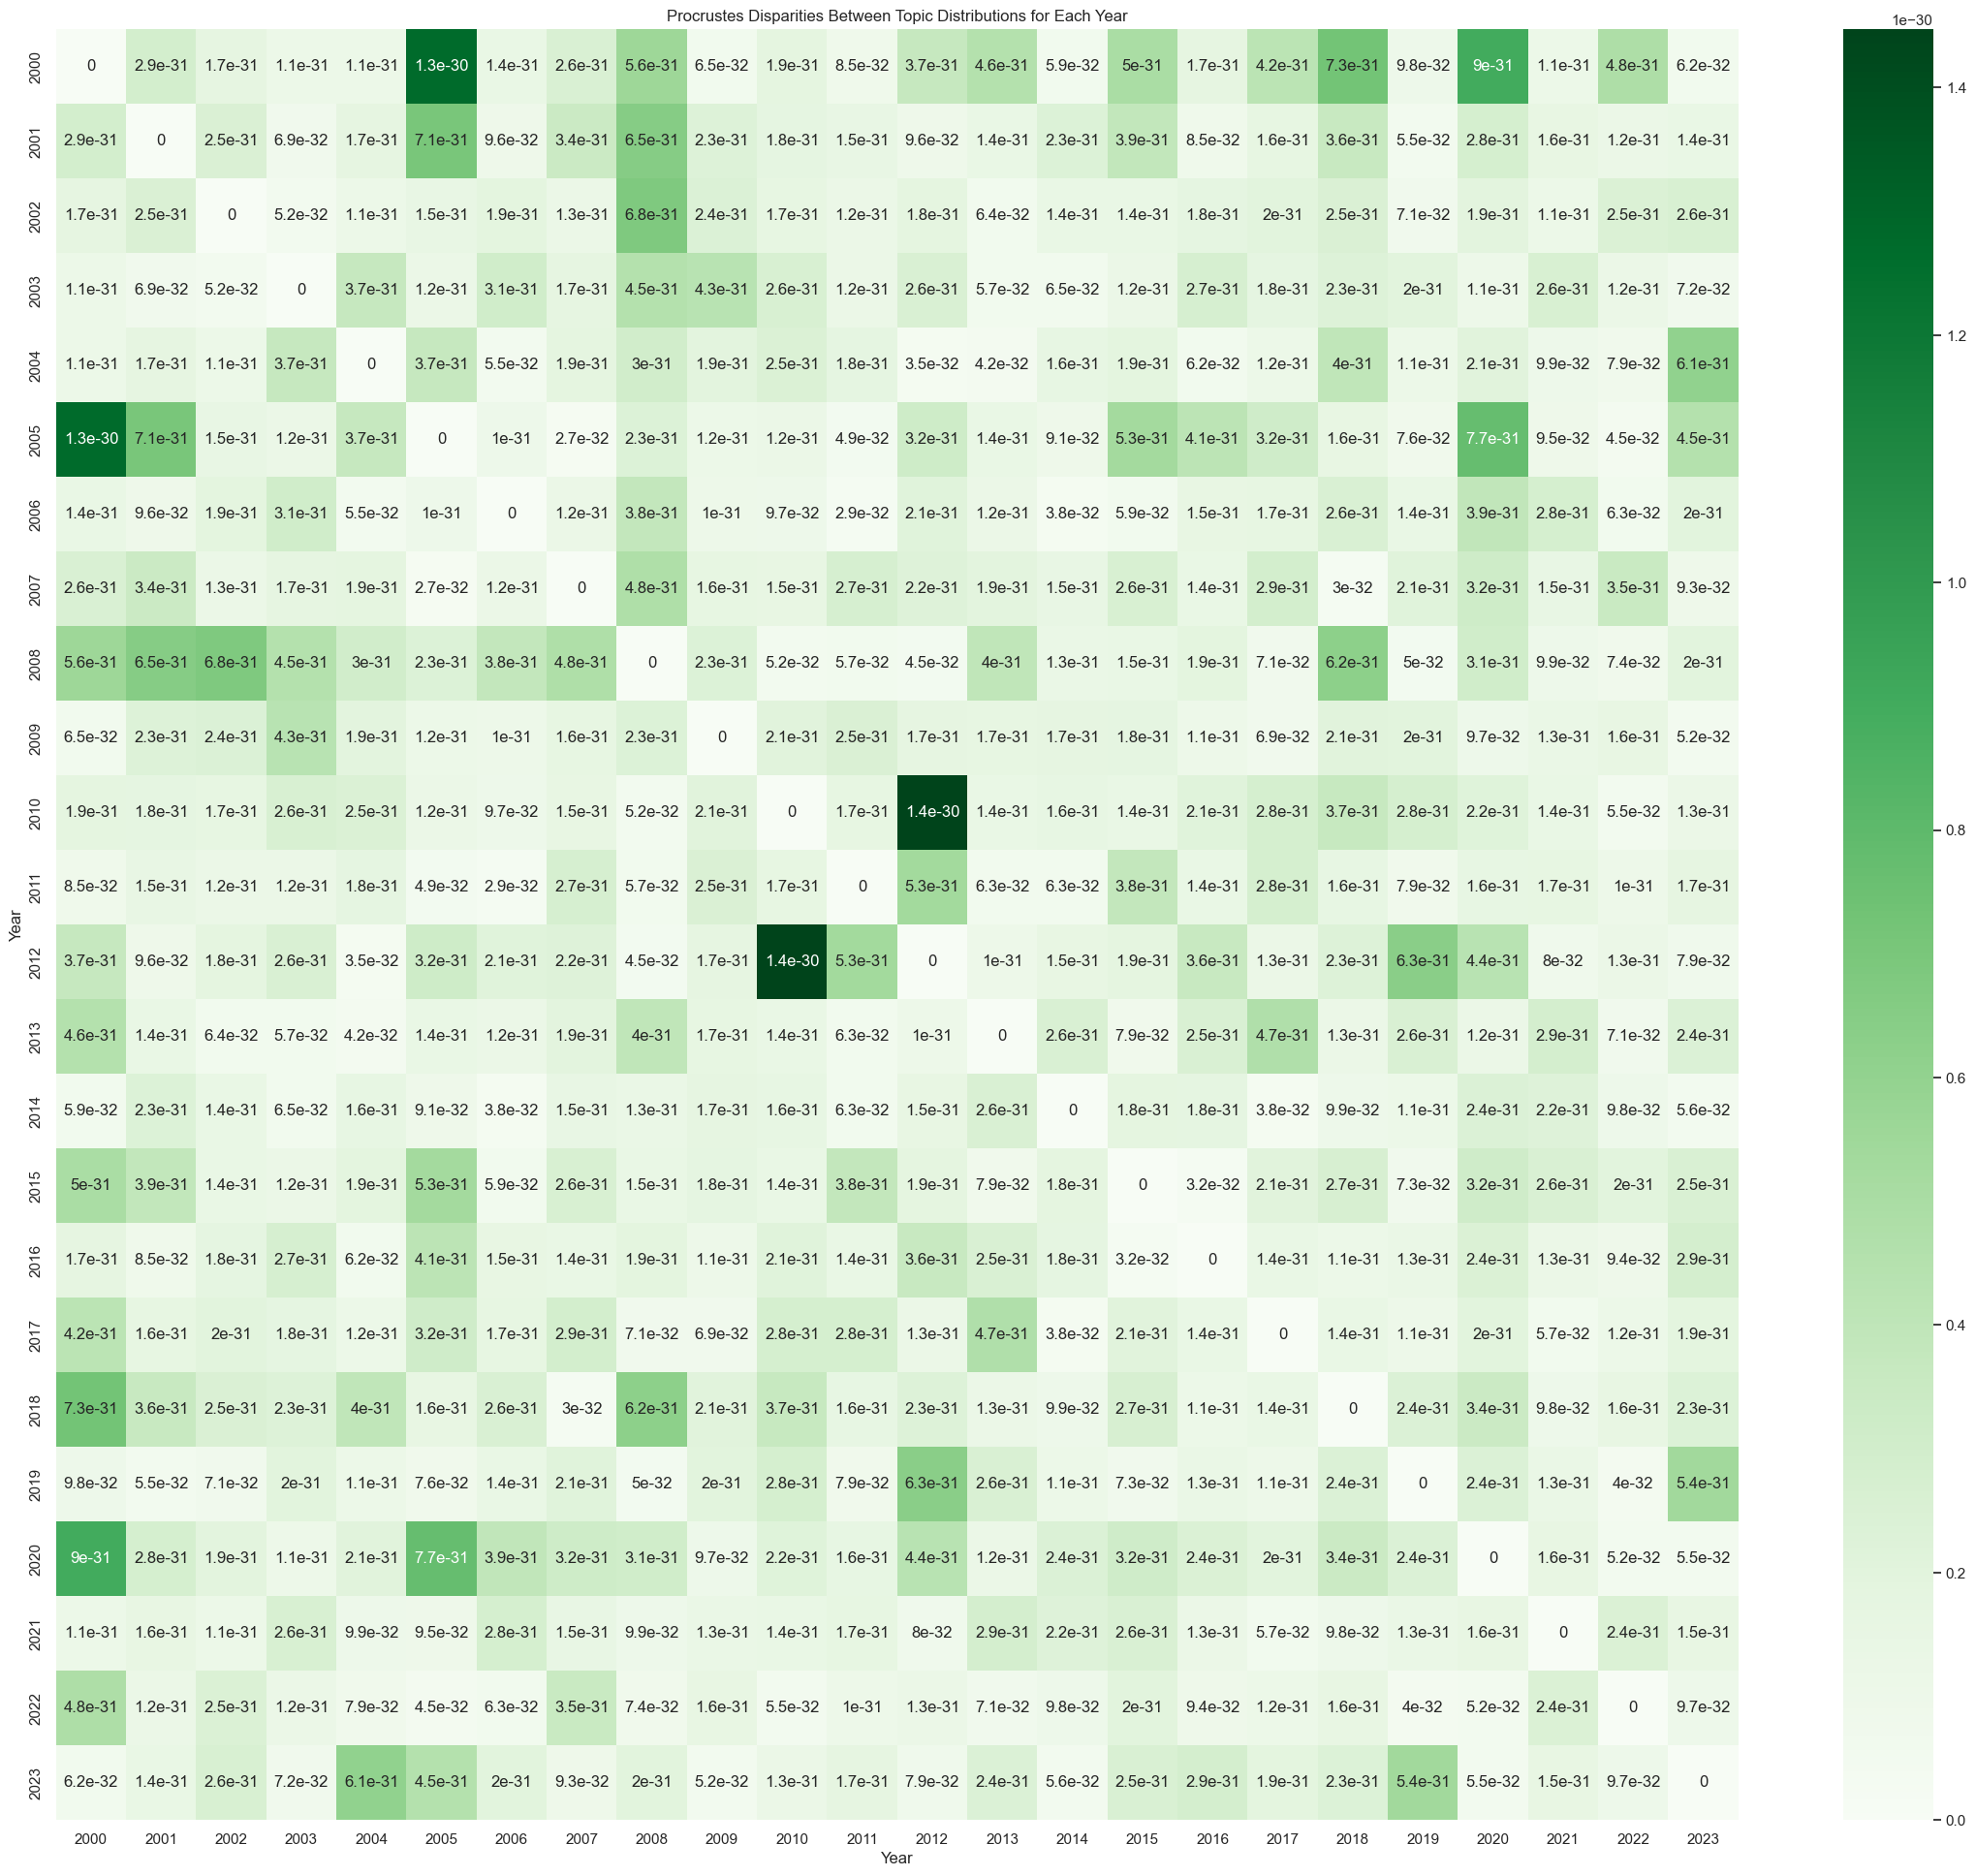
\includegraphics[width=\textwidth]{figures/procrustes/heatmap.png}
  \caption{Procrustes Comparison By Years.}
  \label{fig:procrustes-heatmap}
\end{figure}

Although some standout shifts are visible, the above plot is too dense to be useful.
Thus, we narrow down the study to consecutive years, as shown in~\cref{fig:procrustes-consecutive},
and to years relative to $2022$, as shown in~\cref{fig:procrustes-2022}.
We thought these two studies would be useful to identify both gradual shifts
and shifts relative to the introduction of large language models (LLMs)
in $2020$.

\subsection{Procrustes Analysis of Consecutive Years}~\label{subsec:procrustes-consecutive}

\begin{figure}[H]
  \centering
  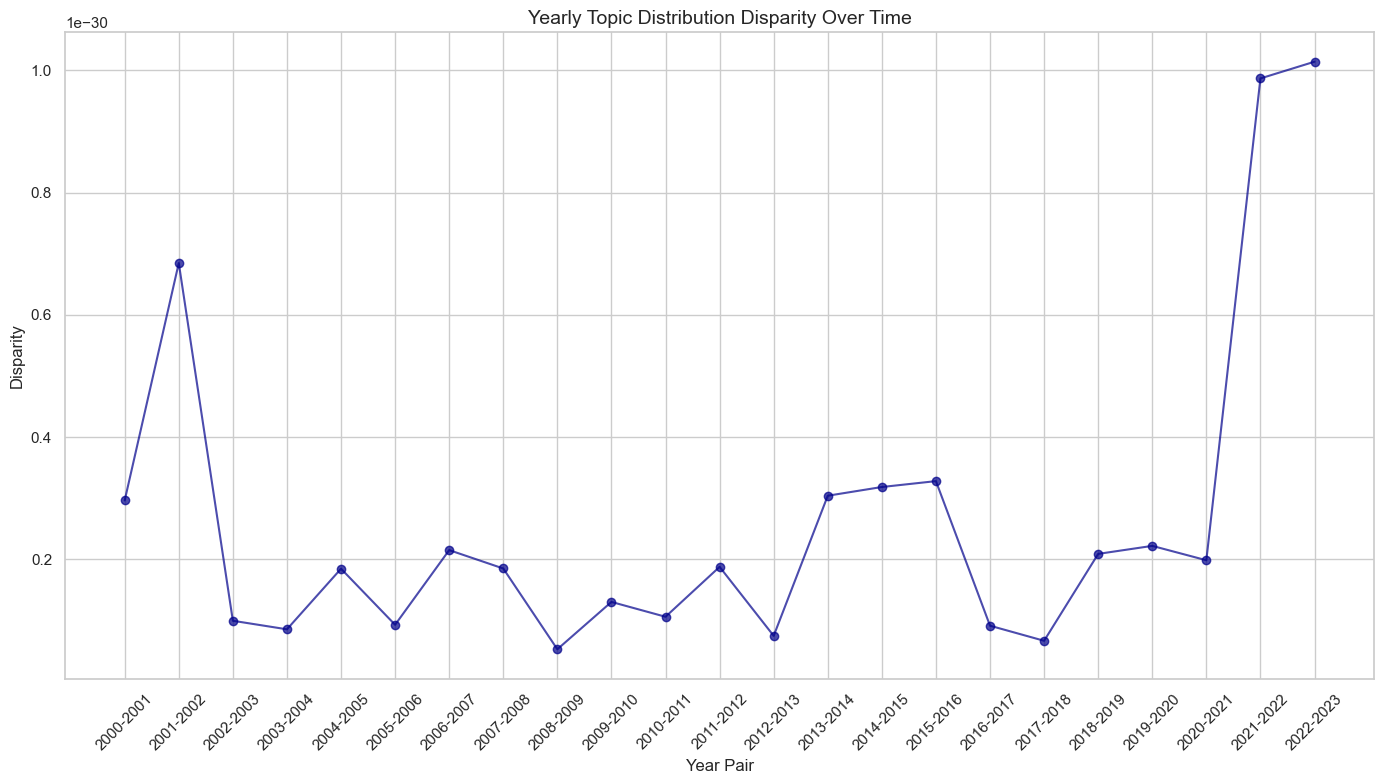
\includegraphics[width=\textwidth]{figures/procrustes/procrustes-consecutive.png}
  \caption{Procrustes analysis of consecutive years.}
  \label{fig:procrustes-consecutive}
\end{figure}

A lower disparity value suggests a higher similarity in topic distributions
(the 10 topics for LDA) from one year to the next, while a higher value denotes a more pronounced change.

We notice a few interesting trends:
\begin{enumroman}
  \item In the early 2000s, there is a relatively minor flucations in disparity.
    However, there appears to be significant shifts in the periods
    $2000$--$2001$ and $2001$--$2002$.
    This period corresponds to the period of the dot-com bubble burst, which may have influenced
    a shift in the discourse around AI, and technology in general.
  \item From $2002$ to around $2013$, there is relatively minor fluctuations in disparity.
  \item There is noticeably higher disparities in the period from $2013$ to $2016$.
    These years could correspond to multiple significant events, such as technological advancements,
    presidential elections, and social-media becoming more mainstream.
  \item From $2018$ onward, we see a \emph{significant} increase in disparity,
    with the highest disparities in $2021$--$2022$ and $2022$--$2023$.
    This three-year period corresponds to the significant advancements in
    language models, such as GPT-3~\cite{gpt3-paper},
    which have been shown to be capable of generating text that is nearly indistinguishable
    from human-written text.
    This could be due to the introduction of LLMs, which have been shown to be
    capable of generating text that is indistinguishable from human-written text.
    This could have caused a shift in the discourse around AI, as people
    became more aware of the capabilities of AI.
\end{enumroman}

\subsection{Procrustes Analysis Relative to 2022}~\label{subsec:procrustes-2022}
To identify gradual shifts, we studied how all years compare to a single year.
We picked $2022$ for this study since it is the year when significant advancements
large language models such as GPT-3~\cite{gpt3-paper} started having
impacts in how people do their work and interact with technology,
especially with the commercialization of chatbots such as
ChatGPT~\cite{chatgpt-info}.

\begin{figure}[H]
  \centering
  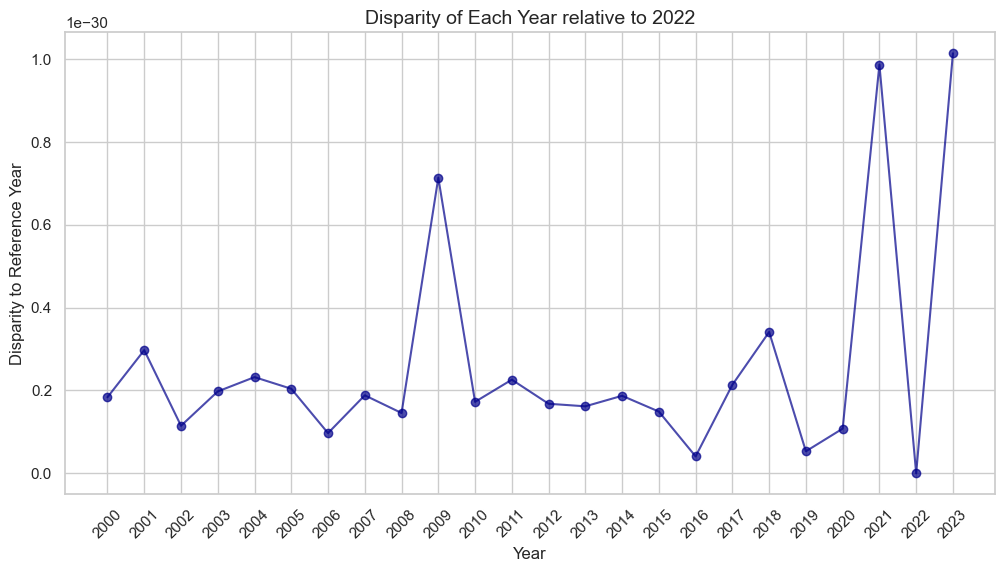
\includegraphics[width=\textwidth]{figures/procrustes/procrustes-2022.png}
  \caption{Procrustes analysis of all years relative to $2022$.}
  \label{fig:procrustes-2022}
\end{figure}

While the disparities are consistently low (compared to the study in~\cref{subsec:procrustes-consecutive}),
it is noticeable that $2009$, $2021$, and $2023$ each have substantial disparities with $2022$.

To understand the reasons for these disparities, we looked at the most-relevant topics
for each of these years, as shown in~\cref{fig:procrustes-topics}.

\newpage
\begin{figure}[H]
  % four plots for 2009, 2021, 2022, and 2023
  \centering
  \begin{subfigure}[b]{0.45\textwidth}
    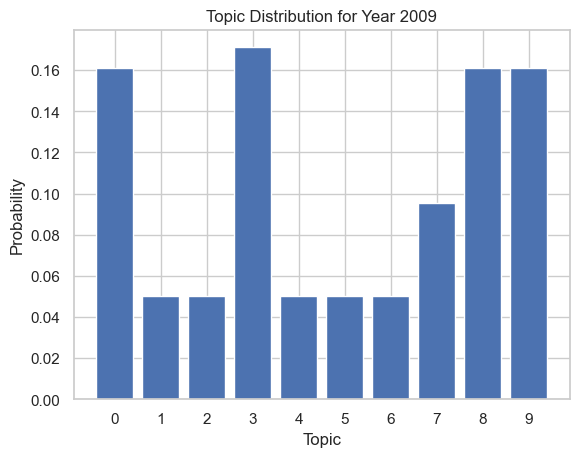
\includegraphics[width=\textwidth]{figures/procrustes/topics-2009.png}
    \caption{Procrustes analysis of $2009$ relative to $2022$.}
    \label{fig:procrustes-topics-2009}
  \end{subfigure}
  \hfill
  \begin{subfigure}[b]{0.45\textwidth}
    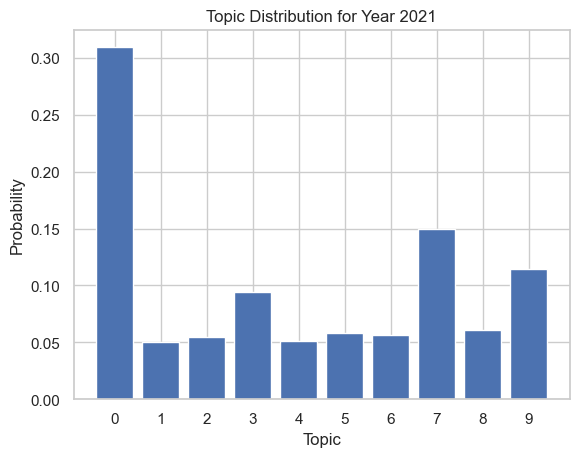
\includegraphics[width=\textwidth]{figures/procrustes/topics-2021.png}
    \caption{Procrustes analysis of $2021$ relative to $2022$.}
    \label{fig:procrustes-topics-2021}
  \end{subfigure}
  \vskip\baselineskip
  \begin{subfigure}[b]{0.45\textwidth}
    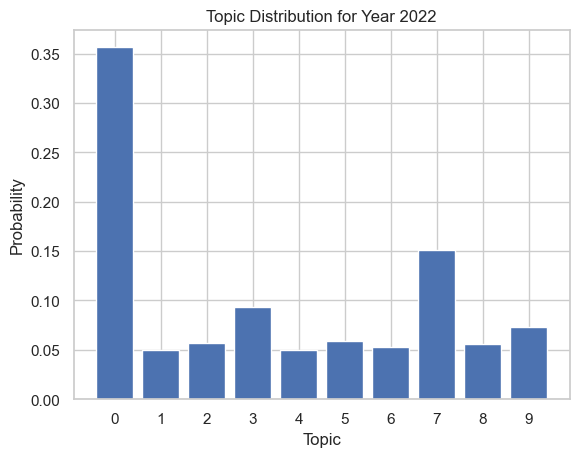
\includegraphics[width=\textwidth]{figures/procrustes/topics-2022.png}
    \caption{Procrustes analysis of $2022$ relative to $2022$.}
    \label{fig:procrustes-topics-2022}
  \end{subfigure}
  \hfill
  \begin{subfigure}[b]{0.45\textwidth}
    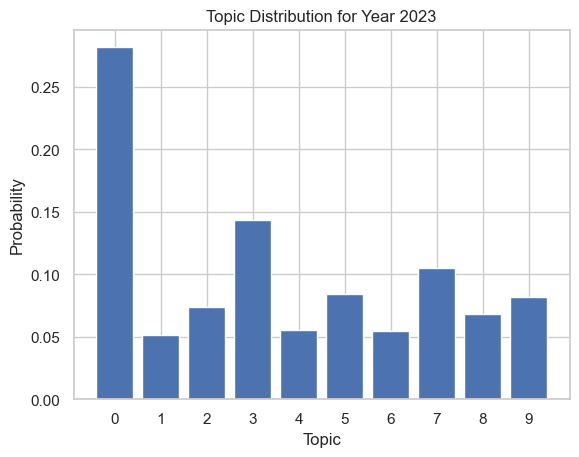
\includegraphics[width=\textwidth]{figures/procrustes/topics-2023.png}
    \caption{Procrustes analysis of $2023$ relative to $2022$.}
    \label{fig:procrustes-topics-2023}
  \end{subfigure}
  \caption{The Most-Relevant Topics for Each of $2009,\ 2021,\ 2022,$ and $2023$.}
  \label{fig:procrustes-topics}
\end{figure}

We notice a few trends:
\begin{enumroman}
  \item \emph{Topic 0} remains nearly most-relevant across both periods.
    When we look at the top words for this topic, they include:
    \emph{model, machine, algorithm, train, research, $\ldots$}.
    It is not surprising that these would occur consistently
    across both periods, since they are fundamental to AI.
  \item \emph{Topic 3} and \emph{Topic 7} also feature consistently among the top topics
    across the years. Their top words include \emph{openai, human, research, think, explain}, and \emph{sam}.
\end{enumroman}
